\PassOptionsToPackage{fontset=none}{ctex}
\PassOptionsToPackage{bookmarks=false}{hyperref}
\documentclass[withoutpreface,bwprint]{cumcmthesis}

\usepackage{cumcm2026}
\usepackage{amsmath,amssymb}
\usepackage{booktabs}
\usepackage{array}
\usepackage{longtable}
\usepackage{siunitx}
\usepackage{graphicx}
\usepackage{placeins}
\usepackage{url}

\sisetup{per-mode=symbol}
\IfFontExistsTF{SimSun}{
  \setCJKmainfont{SimSun}[BoldFont=SimHei]
  \setCJKsansfont{SimHei}[BoldFont=SimHei]
  \setCJKmonofont{FangSong}[BoldFont=SimHei]
  \setCJKfamilyfont{zhsong}{SimSun}[BoldFont=SimHei]
  \setCJKfamilyfont{zhhei}{SimHei}[BoldFont=SimHei]
  \setCJKfamilyfont{zhkai}{KaiTi}[BoldFont=SimHei]
  \setCJKfamilyfont{zhfs}{FangSong}[BoldFont=SimHei]
}{
  \setCJKmainfont{FandolSong-Regular}[BoldFont=FandolHei-Bold]
  \setCJKsansfont{FandolHei-Regular}[BoldFont=FandolHei-Bold]
  \setCJKmonofont{FandolFang-Regular}
  \setCJKfamilyfont{zhsong}{FandolSong-Regular}[BoldFont=FandolHei-Bold]
  \setCJKfamilyfont{zhhei}{FandolHei-Regular}[BoldFont=FandolHei-Bold]
  \setCJKfamilyfont{zhkai}{FandolKai-Regular}
  \setCJKfamilyfont{zhfs}{FandolFang-Regular}
}
\providecommand{\songti}{\CJKfamily{zhsong}}
\providecommand{\heiti}{\CJKfamily{zhhei}}
\providecommand{\kaishu}{\CJKfamily{zhkai}}
\providecommand{\fangsong}{\CJKfamily{zhfs}}

\title{收缩圆柱药材烘干的变物性热质传递建模}

\tihao{A}
\baominghao{}
\schoolname{}
\membera{}
\memberb{}
\memberc{}
\supervisor{}
\yearinput{2026}
\monthinput{9}
\dayinput{11}

\begin{document}

\maketitle

\begin{abstract}
圆柱形中药材在时变烘房边界下同时发生径向升温和失水，预热阶段的非线性扩散使内部场难以由表面状态直接判断。依据轴对称特征建立\textbf{径向有限体积模型}，以分段线性插值重构空气边界，对温度方程作全隐式离散，对水分方程作 Picard 迭代。问题一在一千八百秒得到\textbf{中心与表面温度分别为 33.5756 摄氏度和 36.7857 摄氏度，中心与表面干基含水率分别为 2.5500 千克每千克和 1.5103 千克每千克}。\textbf{表面升温和失水均先于中心，水分扩散前沿在三十分钟内尚未充分到达轴线。}

恒温干燥阶段的密度、比热容、导热系数和水分扩散系数随局部场量变化。构建\textbf{变物性顺序耦合模型}，在每个时间层交替更新温度、含水率和物性，首个时间层采用后向欧拉格式，后续采用二阶向后差分格式。问题二在三小时得到\textbf{中心与表面温度分别为 49.8495 摄氏度和 49.9664 摄氏度，中心与表面干基含水率分别为 1.7662 千克每千克和 1.0081 千克每千克}。\textbf{此时径向温差已缩小至 0.1169 摄氏度，含水率差仍为 0.7581 千克每千克，温度场先于含水率场趋于均匀。}

药材各处含水率均需低于 0.15 千克每千克，固定尺寸模型还需处理附件记录结束后的空气边界。以稳定段九十一个观测值的均值延拓空气状态，并逐秒检查全部径向节点的最大含水率。问题三得到\textbf{固定半径烘干时长为 57.4322 小时}，终点中心含水率的未舍入值为 0.14999973 千克每千克。\textbf{轴线处是固定尺寸条件下的干燥终点控制位置。}在稳定段均值的标准差扰动及末条记录替代情景中，终点时长的最大绝对相对变化为 0.5117\%，空间网格加密所得时长相对差为 0.09044\%。

尺寸收缩使物理域和扩散距离同步变化。将实测半径作为移动边界，建立\textbf{移动材料坐标模型}，在固定单位区间内更新几何权重和附录四物性。问题四得到\textbf{收缩条件下的烘干时长为 51.0775 小时，终点半径为 1.2000 厘米}。同附录四物性的固定半径对照时长为\textbf{129.7964 小时}，\textbf{观测半径收缩使模型终点缩短 78.7189 小时，缩短比例为 60.6480\%}。在所检验的非均匀映射情景中，最大结构偏差为 0.3143\%。空间网格加密和时间步加密的终点差分别为十三秒和零点五秒。

\keywords{药材烘干；径向有限体积；变物性耦合；移动材料坐标；干基含水率}
\end{abstract}

% 2026 年规范不设置目录。

\section{题目概述}

\subsection{问题背景}

中药材进入热风环境后，表面先与烘房空气交换热量和水分，内部温度梯度与含水率梯度随之形成。热量沿温度降低方向传递，水分沿含水率降低方向迁移，两个场共同决定升温速率、失水速率及干燥均匀性。农产品热风干燥研究通常采用干燥动力学模型、连续介质模型或孔道网络模型，连续介质模型能够直接描述物料内部的时空分布\cite{liu2020}。

试验法需要反复改变温度、湿度和干燥时长，完整试验往往覆盖数日。数值模型可在给定物性和边界条件后计算内部场分布，据此筛选工艺参数并识别干燥终点。圆柱物料的对流干燥可用非稳态热传导方程和水分扩散方程描述\cite{tzempelikos2015}，轴对称二维模型还能保留径向及轴向梯度\cite{hussain2003}。

本题所给药材长度为 \SI{25}{cm}，初始半径为 \SI{2}{cm}，观测位置全部由到轴线的距离确定。固定尺寸阶段可在端部影响较弱的条件下化为一维径向问题。已有圆柱形产品研究采用一维有限体积模型同时处理热量和水分交换，并以第三类边界表示表面对流过程\cite{silva2014}。问题四给出随时间变化的半径，需要在前述模型上加入移动边界修正。

\subsection{问题重述}

问题一要求刻画预热平衡阶段的药材温度和干基含水率。烘房温度及空气水分浓度由附件一给出，药材初始温度为 \SI{28}{\degreeCelsius}，初始干基含水率为 \SI{2.55}{kg/kg}。模型需要输出 \SI{1800}{s} 内指定时刻和指定半径位置的温度及含水率，并按 \SI{1}{s} 的时间间隔和 \SI{0.1}{cm} 的空间间隔形成完整结果文件。

问题二把计算范围扩展到预热平衡和恒温干燥阶段，密度、比热容、导热系数和水分扩散系数随含水率或温度变化。论文需要给出前三小时内每隔 \SI{0.5}{h} 的径向温度及含水率。问题三沿用这一变物性模型，以药材所有位置的含水率均低于 \SI{0.15}{kg/kg} 为结束条件，计算固定尺寸假设下的最早干燥时刻。

问题四引入附件二记录的半径变化，并采用附录四给出的物性经验式重新计算干燥时长。空间输出点仍按到轴线的实际距离定义，最外侧输出点随药材表面移动。尺寸效应应通过同样采用附录四物性、仅保持初始半径不变的对照评价；问题三与问题四的差异同时包含物性改变，不能全部归因于收缩。

\section{问题分析}

\subsection{问题一：预热阶段的径向场}

烘房状态每 \SI{60}{s} 记录一次，药材内部结果要求每 \SI{1}{s} 输出一次。离散边界数据需要先转换成连续时间函数，再作为表面对流条件进入控制方程。分段线性插值能够保留每个观测点，并避免高阶插值在相邻记录间产生超调。

药材长径比为 \(L/R=12.5\)，两个端面总面积与侧面积之比为 \(R/L=0.08\)。题目只要求径向位置的结果，因此采用轴对称一维径向模型，忽略轴向梯度。温度场满足 Fourier 导热定律，水分场满足 Fick 扩散定律，表面分别施加对流换热和对流传质边界。

问题一的物性参数均由附录二给定。温度方程为线性扩散方程，水分扩散系数随含水率变化，使水分方程呈非线性。径向有限体积法可直接守恒每个环形控制体内的热量和水分，并利用中心控制体的零面积内边界消除圆柱坐标在轴线处的形式奇点。

\subsection{问题二：全程模型的参数更新}

前三小时处于附件一覆盖的时间范围内，烘房温度和空气水分浓度可以继续采用分段线性插值。附录三把密度、比热容和导热系数写成含水率函数，把扩散系数写成含水率及绝对温度的函数。每个时间层都需依据当前场值更新这些参数，再求解温度场和含水率场。

温度会改变水分扩散系数，含水率又会改变热物性，两个方程通过参数形成顺序耦合。首个时间层采用后向 Euler 格式建立历史状态，其余时间层采用二阶向后差分。每个新时间层内交替更新温度、含水率和物性，直至两类场量的最大绝对变化同时达到容差。

\subsection{问题三：固定尺寸下的干燥终点}

干燥结束条件约束的是药材所有位置，而非某个抽样位置。对每个输出时刻计算径向最大含水率，可以避免未经验证就把中心点当作控制点。若数值结果表明含水率沿半径单调下降，最大值才可由中心含水率代替。

附件一在 \SI{14400}{s} 结束，而问题三的计算范围超过该时刻。取 \SI{9000}{s} 至 \SI{14400}{s} 的九十一个观测点计算稳定段均值，用它延拓后续空气边界。该处理保留平台水平，也削弱单条记录的随机波动。

干燥终点由全域最大含水率首次严格低于 \SI{0.15}{kg/kg} 的时间步确定。程序每秒检查全部径向节点，每隔 \SI{60}{s} 写入结果，并额外保留终点记录。输出频率因此不限制终点的时间分辨率。

\subsection{问题四：收缩边界下的干燥终点}

附件二给出半径从 \SI{2}{cm} 降至 \SI{1.198}{cm} 的离散记录，固定物理坐标上的计算域随时间改变。直接删减外层网格会造成控制体突变，难以保持通量连续。将径向坐标归一化为单位区间后，网格节点保持固定，半径变化通过材料速度和扩散尺度进入控制方程。

附录四给出的物性关系与附录三不同，计算时需要在移动域上同步更新密度、比热容、导热系数和扩散系数。问题四没有重复给出结束阈值，模型承接问题三的 \SI{0.15}{kg/kg} 要求，并以全域最大含水率判定结束。

半径数据在 \SI{259200}{s} 结束，末段已保持 \SI{1.198}{cm}。若计算终点晚于该时刻，阶段模型令半径维持末值，不进行无依据外推。固定尺寸对照与移动域主模型均采用附录四物性，并保持环境、初值及数值算法一致。内部位移未被观测，相似收缩闭合还需在同一外半径下用非均匀映射检验。

\section{模型假设}

\subsection{几何简化}

药材在各截面上视为同轴圆形，初始长度和半径分别取 \SI{0.25}{m} 与 \SI{0.02}{m}。材料内部不设置孔洞、裂纹和局部空腔，温度及含水率只随径向坐标和时间变化。端面面积占换热总表面积的比例为 \(R/(L+R)\)，其数值约为 \(0.074\)，阶段模型忽略端部通量。

问题一至问题三把药材半径视为常数。问题四只考虑附件二给出的径向收缩，长度保持 \SI{0.25}{m}。半径在相邻观测时刻之间作分段线性变化，归一化坐标下的圆柱仍保持轴对称。题面未提供内部位移和干固体密度的闭合关系，故采用随材料运动的有效标量扩散模型。面积加权含水率只作几何平均诊断，不解释为已经验证的真实水分质量库存。

\subsection{材料状态}

任一时刻的同一径向控制体内视为均匀连续介质，局部温度和干基含水率可以用单值函数表示。问题一采用附录二中的常密度、常比热容和常导热系数，问题二至问题四按题面经验式逐点更新物性。

模型不计内部化学反应热、辐射换热和药材与托盘之间的接触传热。水分迁移用等效液态扩散描述，气液相变过程及毛细输运统一折算到题面给出的有效扩散系数中。蒸发潜热没有单列为温度方程源项，这一处理会在模型评价中作为适用边界说明。

\subsection{表面交换}

烘房空气在药材表面附近视为空间均匀，附件一的温度和水分浓度可代表整段侧壁的环境状态。表面对流换热系数和对流传质系数在问题一中取附录二数值，表面不存在额外热阻和质阻。

题面把药材干基含水率和空气水分浓度均记为 \si{kg/kg}。阶段模型按题设口径直接用二者差值构造传质驱动力，不再转换平衡含水率。该处理等价于采用题面给定的经验边界，最终稿需根据数值合理性复核量纲基准。

问题三在附件一结束后采用稳定段均值作为空气边界。温度取 \SI{50.004945}{\degreeCelsius}，空气水分浓度取 \SI{0.049993736}{kg/kg}。稳定段总体标准差及末条记录替代工况用于检验这一延拓对终点时长的影响。

\subsection{数值离散}

径向控制体边界与轴线同心，单元内物性由节点值代表。控制面导热系数取相邻节点值的算术平均，水分扩散系数采用同样规则。问题一采用全隐式时间格式，问题二从第二个时间层起采用二阶向后差分，非线性物性在单个时间层内迭代更新。

问题一的权威内部网格取 \(\Delta r=\SI{0.000125}{m}\)，时间步取 \(\Delta t=\SI{0.25}{s}\)。程序每隔 \SI{1}{s} 保存一次，并把内部节点插值到题目要求的 \SI{0.1}{cm} 空间间隔。问题二沿用 \SI{1}{s} 输出间隔。问题三采用三百二十个径向区间和 \SI{1}{s} 时间步，每隔 \SI{60}{s} 保存一次，并保留终点短步。空间网格及时间步加密结果用于检验离散精度。

\section{符号说明}

温度统一以绝对温度进入控制方程和扩散系数，表格输出时再换算为摄氏温度。含水率采用题目给出的干基定义。表 \ref{tab:symbols} 列出正文使用的核心符号，离散上下标只在有限体积小节内解释。

\begin{longtable}{>{\centering\arraybackslash}p{0.16\textwidth}
                  p{0.56\textwidth}
                  >{\centering\arraybackslash}p{0.16\textwidth}}
\caption{主要符号及含义}\label{tab:symbols}\\
\toprule
符号 & 含义 & 单位\\
\midrule
\endfirsthead
\toprule
符号 & 含义 & 单位\\
\midrule
\endhead
\bottomrule
\endfoot
\(t\) & 烘干开始后的时间 & \si{s}\\
\(r\) & 到药材轴线的径向距离 & \si{m}\\
\(x\) & 收缩模型中的归一化径向坐标 & 1\\
\(\xi\) & 非均匀收缩模型中的材料坐标 & 1\\
\(L\) & 药材长度 & \si{m}\\
\(R\) & 固定尺寸模型中的药材半径 & \si{m}\\
\(R(t)\) & 收缩模型中的药材半径 & \si{m}\\
\(r_\xi\) & 材料映射关于 \(\xi\) 的雅可比 & \si{m}\\
\(a_*\) & 内部非均匀收缩的结构参数 & 1\\
\(T(r,t)\) & 药材绝对温度 & \si{K}\\
\(T_{\mathrm{c}}(r,t)\) & 药材摄氏温度 & \si{\degreeCelsius}\\
\(T_a(t)\) & 烘房空气绝对温度 & \si{K}\\
\(C(r,t)\) & 药材干基含水率 & \si{kg/kg}\\
\(C_a(t)\) & 烘房空气水分浓度 & \si{kg/kg}\\
\(\rho\) & 药材密度 & \si{kg/m^3}\\
\(c_p\) & 药材比热容 & \si{J/(kg.K)}\\
\(k\) & 药材导热系数 & \si{W/(m.K)}\\
\(D\) & 有效水分扩散系数 & \si{m^2/s}\\
\(h\) & 表面对流换热系数 & \si{W/(m^2.K)}\\
\(h_m\) & 表面对流传质系数 & \si{m/s}\\
\(V_i\) & 第 \(i\) 个径向控制体体积 & \si{m^3}\\
\(A_{i+\frac12}\) & 相邻控制体之间的控制面面积 & \si{m^2}\\
\(\Delta r\) & 径向网格步长 & \si{m}\\
\(\Delta t\) & 时间步长 & \si{s}\\
\end{longtable}

式中 \(T_{\mathrm{c}}=T-273.15\)。当正文给出附件一的原始温度时使用摄氏温度，代入附录三和附录四的 Arrhenius 型扩散系数时使用绝对温度，避免因温标混用造成数量级错误。

\section{模型求解}

\subsection{问题一的径向场求解}

\subsubsection{问题一的几何简化}

二维轴对称圆柱模型把温度和含水率写成 \(T(r,z,t)\) 与 \(C(r,z,t)\)，侧壁和端面分别设置对流边界\cite{hussain2003}。题目没有给出轴向观测位置，所有输出点均由到轴线的距离确定。端面总面积与侧面积之比为
\begin{equation}
\frac{2\pi R^2}{2\pi RL}=\frac{R}{L}=0.08.
\label{eq:end-side-ratio}
\end{equation}
端部通量对总体交换面积的贡献受限，故把固定尺寸药材近似为一维径向圆柱。

降维后定义
\begin{equation}
T=T(r,t),\qquad C=C(r,t),\qquad 0\leq r\leq R.
\label{eq:q1-fields}
\end{equation}
式 \ref{eq:q1-fields} 保留径向梯度，能够直接输出题目指定的五个位置。该简化不代表轴向温差恒为零，最终需要以二维抽样计算或端部敏感性试验评估其误差。

% 待插图：圆柱药材、径向坐标和表面对流边界示意图。

\subsubsection{问题一的温度模型}

半径为 \(r\) 的圆柱面上，向外径向热流密度满足 Fourier 定律
\begin{equation}
q_r=-k\frac{\partial T}{\partial r}.
\label{eq:fourier}
\end{equation}
将式 \ref{eq:fourier} 代入环形微元的能量守恒关系，得到一维径向非稳态导热方程
\begin{equation}
\rho c_p\frac{\partial T}{\partial t}
=
\frac{1}{r}\frac{\partial}{\partial r}
\left(
r k\frac{\partial T}{\partial r}
\right),
\qquad 0<r<R.
\label{eq:heat-pde}
\end{equation}

问题一取
\begin{equation}
\rho=\SI{820}{kg/m^3},\qquad
c_p=\SI{2600}{J/(kg.K)},\qquad
k=\SI{0.36}{W/(m.K)}.
\label{eq:q1-thermal-properties}
\end{equation}
药材初始温度为
\begin{equation}
T(r,0)=\SI{301.15}{K}.
\label{eq:heat-initial}
\end{equation}
轴线处由对称性得到零梯度条件
\begin{equation}
\left.\frac{\partial T}{\partial r}\right|_{r=0}=0.
\label{eq:heat-center}
\end{equation}

表面热流由烘房空气和药材表面的温差驱动，故有
\begin{equation}
-k\left.\frac{\partial T}{\partial r}\right|_{r=R}
=h\left[T(R,t)-T_a(t)\right],
\qquad h=\SI{25}{W/(m^2.K)}.
\label{eq:heat-surface}
\end{equation}
附件一给出的摄氏温度先作分段线性插值。若 \(t_j\leq t\leq t_{j+1}\)，则
\begin{equation}
T_a(t)
=273.15+T_{a,j}^{\mathrm{c}}
+\frac{T_{a,j+1}^{\mathrm{c}}-T_{a,j}^{\mathrm{c}}}
{t_{j+1}-t_j}
\left(t-t_j\right).
\label{eq:air-temperature-interpolation}
\end{equation}
式 \ref{eq:air-temperature-interpolation} 保证记录时刻的边界值与附件一完全一致。

附件一在预热阶段的原始记录如图 \ref{fig:q1-air-boundary} 所示。三十分钟内，烘房温度由 \SI{28}{\degreeCelsius} 升至 \SI{41.545}{\degreeCelsius}，空气水分浓度由 \SI{0.01963}{kg/kg} 升至 \SI{0.03299}{kg/kg}。两条边界曲线均保留观测点之间的局部斜率变化，没有用单一升温速率替代实测过程。

\begin{figure}[htbp]
\centering
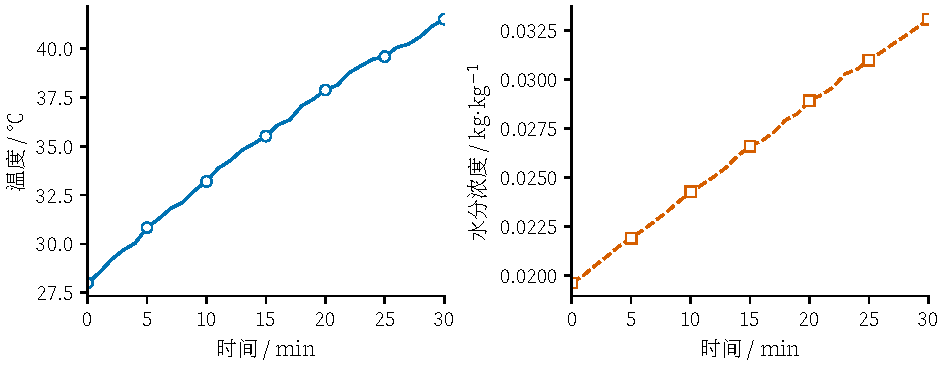
\includegraphics[width=0.92\textwidth]{figures/raw_q1_air_boundary.pdf}
\caption{问题一烘房环境边界的原始记录}
\label{fig:q1-air-boundary}
\end{figure}

\subsubsection{问题一的水分模型}

把 \(C(r,t)\) 定义为药材干基含水率，归一化水分通量写为
\begin{equation}
J_C=-D(C)\frac{\partial C}{\partial r}.
\label{eq:fick}
\end{equation}
环形微元内的水分守恒给出
\begin{equation}
\frac{\partial C}{\partial t}
=
\frac{1}{r}\frac{\partial}{\partial r}
\left[
rD(C)\frac{\partial C}{\partial r}
\right],
\qquad 0<r<R.
\label{eq:moisture-pde}
\end{equation}
附录二的经验式应按题面写为
\begin{equation}
D(C)
=7\times 10^{-9}
\exp\left(-\frac{0.89}{C}\right).
\label{eq:q1-diffusivity}
\end{equation}

式 \ref{eq:q1-diffusivity} 的指数含 \(C\) 的倒数。含水率下降时，指数项随之减小，有效扩散系数降低，模型由此描述低含水率阶段逐渐增大的内部迁移阻力。水分初始条件和轴线边界为
\begin{equation}
C(r,0)=2.55,\qquad
\left.\frac{\partial C}{\partial r}\right|_{r=0}=0.
\label{eq:moisture-initial-center}
\end{equation}
% 输入核验备注：Q1 原稿把指数误写为 -0.89C，后续不得恢复该写法。

药材表面采用第三类传质边界
\begin{equation}
-D(C)\left.\frac{\partial C}{\partial r}\right|_{r=R}
=h_m\left[C(R,t)-C_a(t)\right],
\qquad h_m=8\times10^{-7}\ \si{m/s}.
\label{eq:moisture-surface}
\end{equation}
附件一中的空气水分浓度按式 \ref{eq:air-temperature-interpolation} 的同类形式作分段线性插值。该边界按题设统一浓度口径，控制表面水分离开药材的速率。

\subsubsection{问题一的数值求解}

在 \(0\leq r\leq R\) 上设置节点 \(r_i=i\Delta r\)，其中 \(i=0,1,\ldots,N\)。节点两侧控制面为 \(r_{i-\frac12}\) 与 \(r_{i+\frac12}\)。内部控制体体积及控制面面积分别为
\begin{align}
V_i&=\pi L
\left(
r_{i+\frac12}^{2}-r_{i-\frac12}^{2}
\right),\\
A_{i\pm\frac12}&=2\pi Lr_{i\pm\frac12}.
\label{eq:fvm-geometry}
\end{align}
中心控制体取 \(0\leq r\leq \Delta r/2\)，其内侧控制面面积为零。表面控制体取 \(R-\Delta r/2\leq r\leq R\)。

时间层记为 \(t_n=n\Delta t\)。内部节点的全隐式温度离散式为
\begin{align}
\frac{\rho c_pV_i}{\Delta t}
\left(T_i^{n+1}-T_i^n\right)
={}&
\frac{kA_{i-\frac12}}{\Delta r}
\left(T_{i-1}^{n+1}-T_i^{n+1}\right)\notag\\
&+
\frac{kA_{i+\frac12}}{\Delta r}
\left(T_{i+1}^{n+1}-T_i^{n+1}\right).
\label{eq:heat-fvm}
\end{align}
中心节点只保留外侧控制面通量，表面节点在内侧导热通量外加入
\begin{equation}
hA_R\left(T_a^{n+1}-T_N^{n+1}\right),
\qquad A_R=2\pi RL.
\label{eq:surface-heat-flux}
\end{equation}
由此得到包含 \(T_0^{n+1}\) 至 \(T_N^{n+1}\) 的完整三对角方程组。

水分方程采用相同控制体。第 \(\ell\) 次非线性迭代中，以当前含水率计算
\begin{equation}
D_{i+\frac12}^{(\ell)}
=
\frac{
D\left(C_i^{(\ell)}\right)
+D\left(C_{i+1}^{(\ell)}\right)
}{2},
\label{eq:interface-diffusivity}
\end{equation}
再求解
\begin{align}
\frac{V_i}{\Delta t}
\left(C_i^{n+1,\ell+1}-C_i^n\right)
={}&
\frac{D_{i-\frac12}^{(\ell)}A_{i-\frac12}}{\Delta r}
\left(C_{i-1}^{n+1,\ell+1}-C_i^{n+1,\ell+1}\right)\notag\\
&+
\frac{D_{i+\frac12}^{(\ell)}A_{i+\frac12}}{\Delta r}
\left(C_{i+1}^{n+1,\ell+1}-C_i^{n+1,\ell+1}\right).
\label{eq:moisture-fvm}
\end{align}
表面控制体再加入
\begin{equation}
-h_mA_R\left(C_N^{n+1,\ell+1}-C_a^{n+1}\right).
\label{eq:surface-moisture-flux}
\end{equation}
相邻两次迭代的含水率最大差不超过 \(10^{-10}\) 后进入下一时间层，单步最多迭代五十次。计算过程中实际最多进行四次迭代，全部时间层均达到收敛容差。线性方程组采用 Thomas 算法求解，权威网格下热量矩阵与水分矩阵的条件数分别为 \(1.889\times10^3\) 和 \(1.254\times10^3\)，均低于病态判据 \(10^7\)。

权威计算取 \(\Delta r=\SI{0.000125}{m}\) 与 \(\Delta t=\SI{0.25}{s}\)，对应一百六十个径向小区间和七千二百个时间步。程序每隔四个内部时间步输出一次，并将内部网格线性抽取到题目要求的 \SI{0.1}{cm} 间隔。温度以摄氏度输出，全部结果按题目模板保留四位小数。

% 待插图：径向有限体积网格及中心、表面控制体。

\subsubsection{问题一的模型计算结果}

表 \ref{tab:q1-temperature} 与表 \ref{tab:q1-moisture} 给出题目指定位置的计算值。药材表面温度在 \SI{1800}{s} 时达到 \SI{36.7857}{\degreeCelsius}，中心温度为 \SI{33.5756}{\degreeCelsius}，径向温差为 \SI{3.2101}{\degreeCelsius}。同一时刻表面含水率降至 \SI{1.5103}{kg/kg}，中心含水率按四位小数仍为 \SI{2.5500}{kg/kg}，失水前沿尚未充分到达轴线。

\begin{table}[htbp]
\centering
\caption{三十分钟内药材温度}
\label{tab:q1-temperature}
\small
\begin{tabular}{cccccc}
\toprule
时间 & \multicolumn{5}{c}{距轴线距离对应温度 \si{\degreeCelsius}} \\
\cmidrule(lr){2-6}
\si{s} & \SI{0}{cm} & \SI{0.5}{cm} & \SI{1}{cm} & \SI{1.5}{cm} & \SI{2}{cm} \\
\midrule
100  & 28.0001 & 28.0004 & 28.0041 & 28.0328 & 28.1802 \\
300  & 28.0410 & 28.0637 & 28.1516 & 28.3683 & 28.8491 \\
600  & 28.4537 & 28.5364 & 28.8043 & 29.3162 & 30.1654 \\
900  & 29.3248 & 29.4587 & 29.8759 & 30.6165 & 31.7306 \\
1200 & 30.5432 & 30.7102 & 31.2227 & 32.1129 & 33.4279 \\
1500 & 31.9961 & 32.1871 & 32.7664 & 33.7465 & 35.1204 \\
1800 & 33.5756 & 33.7723 & 34.3644 & 35.3624 & 36.7857 \\
\bottomrule
\end{tabular}
\end{table}

\begin{table}[htbp]
\centering
\caption{三十分钟内药材干基含水率}
\label{tab:q1-moisture}
\small
\begin{tabular}{cccccc}
\toprule
时间 & \multicolumn{5}{c}{距轴线距离对应含水率 \si{kg/kg}} \\
\cmidrule(lr){2-6}
\si{s} & \SI{0}{cm} & \SI{0.5}{cm} & \SI{1}{cm} & \SI{1.5}{cm} & \SI{2}{cm} \\
\midrule
100  & 2.5500 & 2.5500 & 2.5500 & 2.5500 & 2.2476 \\
300  & 2.5500 & 2.5500 & 2.5500 & 2.5492 & 2.0511 \\
600  & 2.5500 & 2.5500 & 2.5500 & 2.5352 & 1.8771 \\
900  & 2.5500 & 2.5500 & 2.5497 & 2.5045 & 1.7548 \\
1200 & 2.5500 & 2.5500 & 2.5482 & 2.4646 & 1.6586 \\
1500 & 2.5500 & 2.5499 & 2.5445 & 2.4206 & 1.5788 \\
1800 & 2.5500 & 2.5497 & 2.5383 & 2.3755 & 1.5103 \\
\bottomrule
\end{tabular}
\end{table}

图 \ref{fig:q1-fields} 展示完整时空场。温度响应从外表面向轴线逐渐传播，含水率下降集中在靠近表面的区域，两个场的扩散深度存在差异。温度边界与内部场的响应方向一致，含水率始终由内部向表面递减，表面对流项的符号与物理过程相符。

\begin{figure}[htbp]
\centering
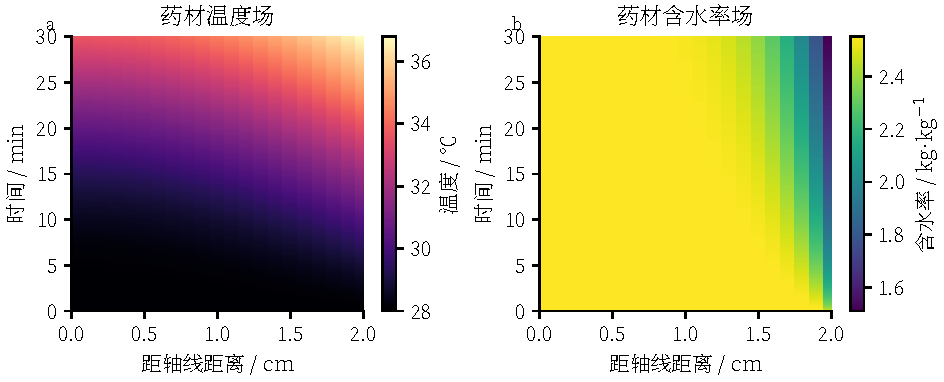
\includegraphics[width=0.92\textwidth]{figures/result_q1_fields.pdf}
\caption{问题一温度场与干基含水率场}
\label{fig:q1-fields}
\end{figure}

将时间步缩小至 \SI{0.125}{s} 后，指定时空点的温度与含水率最大绝对差分别为 \(2.389\times10^{-4}\) \si{\degreeCelsius} 和 \(5.139\times10^{-5}\) \si{kg/kg}。将空间步缩小至 \SI{0.0000625}{m} 后，对应差值分别为 \(2.300\times10^{-5}\) \si{\degreeCelsius} 和 \(3.505\times10^{-4}\) \si{kg/kg}。图 \ref{fig:q1-convergence} 给出两类加密误差，含水率对表面附近的空间分辨率更敏感。

\begin{figure}[htbp]
\centering
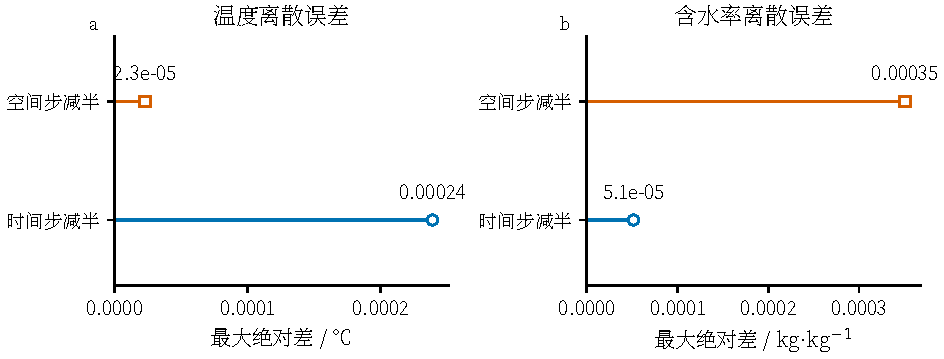
\includegraphics[width=0.92\textwidth]{figures/process_q1_convergence.pdf}
\caption{问题一数值加密误差}
\label{fig:q1-convergence}
\end{figure}

由控制体内含水率总变化与表面对流通量分别计算整体平衡，所得相对残差为 \(2.35\times10^{-14}\)。该数值接近双精度浮点运算的舍入尺度，说明离散方程中的内部通量能够在相邻控制体之间抵消，表面通量与域内总量变化保持一致。

\subsection{问题二的全程变物性模型}

附件一在前三小时内提供一百八十一条环境记录，采样间隔为 \SI{60}{s}。计算时刻始终落在实测区间内，空气温度 \(T_a(t)\) 和空气水分浓度 \(C_a(t)\) 均由相邻记录线性插值得到。图 \ref{fig:q2-boundary} 显示两类边界量总体上升并伴随逐分钟波动，\SI{3}{h} 时的观测值分别为 \SI{50.195}{\degreeCelsius} 和 \SI{0.04977}{kg/kg}。

\begin{figure}[htbp]
\centering
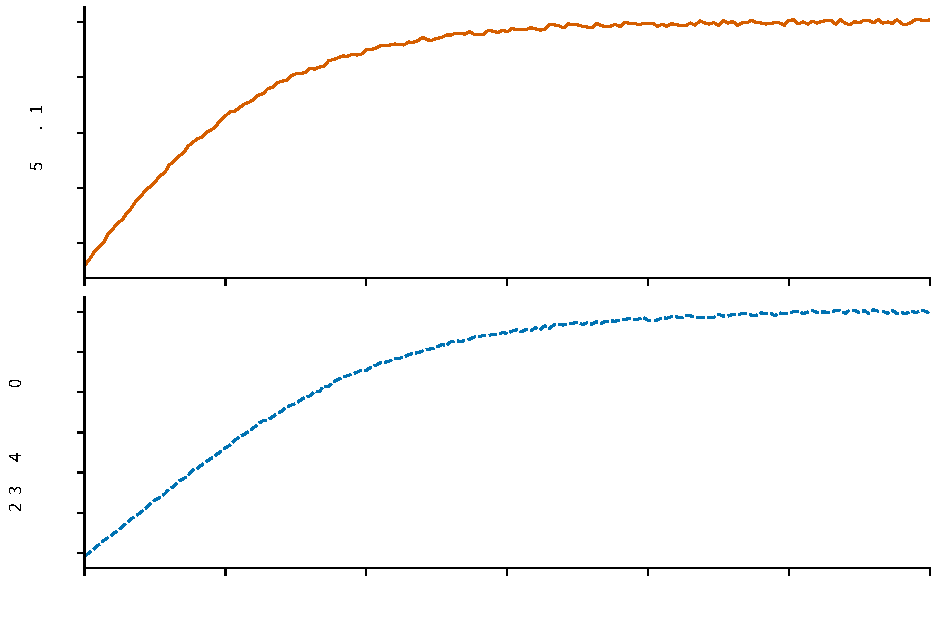
\includegraphics[width=0.92\textwidth]{figures/raw_q2_boundary_series.pdf}
\caption{问题二前三小时的空气边界}
\label{fig:q2-boundary}
\end{figure}

附录三没有另行给出表面对流系数，计算沿用附录二的 \(h=\SI{25}{W/(m^2.K)}\) 和 \(h_m=8\times10^{-7}\,\si{m/s}\)。这项处理属于新增假设，故在基准结果外分别把两个系数调整为原值的 \SI{80}{\percent} 和 \SI{120}{\percent}，检验边界参数对内部场的影响。

\subsubsection{物性反馈机制}

附录三把密度、比热容和导热系数写成局部含水率的函数，并令水分扩散系数同时受含水率和温度控制。各关系式为
\begin{align}
\rho(C)&=650+128C,\label{eq:q2-rho}\\
c_p(C)&=1450+2736\frac{C}{C+1},\label{eq:q2-cp}\\
k(C)&=0.21+0.38\frac{C}{C+1},\label{eq:q2-k}\\
D(C,T)&=2.4\times10^{-3}
\exp\left(-\frac{0.45}{C}\right)
\exp\left(-\frac{3850}{T}\right).
\label{eq:q2-properties}
\end{align}
式 \ref{eq:q2-properties} 中的 \(T\) 采用 K。每次 Picard 迭代先用当前含水率更新 \(\rho\)、\(c_p\) 和 \(k\)，再用更新后的温度和含水率计算 \(D\)。

三小时计算中，\(\rho\) 的取值范围为 \(779.0391\) 至 \(976.4000\,\si{kg/m^3}\)，\(c_p\) 为 \(2823.5301\) 至 \(3415.2958\,\si{J/(kg.K)}\)，\(k\) 为 \(0.400768\) 至 \(0.482958\,\si{W/(m.K)}\)。扩散系数 \(D\) 处于 \(5.5475\times10^{-9}\) 至 \(1.2522\times10^{-8}\,\si{m^2/s}\)。这些数值在计算域内保持有限且为正，离散系统没有出现物性奇点。

\subsubsection{局部守恒方程}

从每个环形控制体的积分平衡出发，可把温度方程和水分方程写成统一形式
\begin{equation}
\beta_i^{n+1,m}V_i\delta_t u_i^{n+1,m+1}
=
\sum_{f=i\pm\frac{1}{2}}
\frac{\Gamma_f^{n+1,m}A_f}{\Delta r}
\left(
u_{\operatorname{nb}(f)}^{n+1,m+1}
-u_i^{n+1,m+1}
\right).
\label{eq:q2-fvm-unified}
\end{equation}
温度方程取 \(u=T\)、\(\beta=\rho c_p\)、\(\Gamma=k\)，水分方程取 \(u=C\)、\(\beta=1\)、\(\Gamma=D\)。相邻节点的物性算术平均值代表控制面物性，同一内部控制面的通量在相邻控制体中符号相反，求和后能够抵消。

轴线控制面的面积为零，式 \ref{eq:q2-fvm-unified} 自然满足对称条件。表面控制体把外侧通量改写为
\begin{equation}
S_{T,N}=hA_R\left(T_a-T_N\right),\qquad
S_{C,N}=-h_mA_R\left(C_N-C_a\right).
\label{eq:q2-surface-sources}
\end{equation}
空气温度高于表面温度时，热源项为正。表面含水率高于空气水分浓度时，水分源项为负，两类符号均与药材升温和失水的方向一致。

\subsubsection{时间层内迭代}

首个时间层采用后向 Euler 格式，得到二阶格式需要的第二个历史状态。从第二个时间层起，式 \ref{eq:q2-fvm-unified} 中的时间导数采用
\begin{equation}
\delta_t u_i^{n+1}
=
\frac{3u_i^{n+1}-4u_i^n+u_i^{n-1}}{2\Delta t}.
\label{eq:q2-bdf2}
\end{equation}
每次物性固定后，温度和含水率各形成一个三对角线性系统，并用追赶法求解。

同一时间层内依次更新温度、扩散系数、含水率和热物性。当相邻两轮温度的最大绝对差低于 \(10^{-8}\,\si{\degreeCelsius}\)，且含水率的最大绝对差低于 \(10^{-10}\,\si{kg/kg}\) 时停止迭代。程序把迭代上限设为四十次，实际有四千二百九十个时间层经过三次迭代收敛，六千五百一十个时间层经过四次迭代收敛，未触及上限。图 \ref{fig:q2-picard} 给出全过程记录。

\begin{figure}[htbp]
\centering
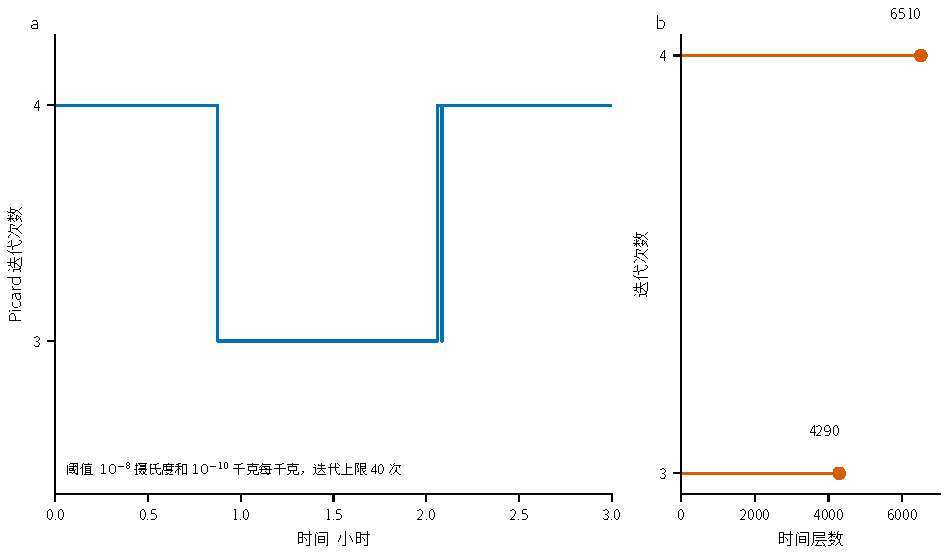
\includegraphics[width=0.92\textwidth]{figures/process_q2_picard_iterations.pdf}
\caption{问题二各时间层的 Picard 迭代次数}
\label{fig:q2-picard}
\end{figure}

权威计算把半径等分为一百六十个区间，\(\Delta r=\SI{0.000125}{m}\)，时间步取 \(\Delta t=\SI{1}{s}\)。程序保存一秒至一万零八百秒的每个时间层，并把内部解线性插值到零至二厘米的二十一个输出位置，空间间隔为 \SI{0.1}{cm}。温度表和水分浓度表各含一万零八百行数据及二十二列，表中数值保留四位小数。

\subsubsection{径向场结果}

表 \ref{tab:q2-temperature} 和表 \ref{tab:q2-moisture} 选取六个时刻及五个径向位置。选定位置覆盖轴线、内层、外层和表面，可直接观察场量从边界向内部传播的过程。

\begin{table}[htbp]
\centering
\caption{问题二指定时空点的温度}
\label{tab:q2-temperature}
\begin{tabular}{cccccc}
\toprule
时间 & \multicolumn{5}{c}{不同半径处温度 \si{\degreeCelsius}}\\
\cmidrule(lr){2-6}
\si{h} & \SI{0}{cm} & \SI{0.5}{cm} & \SI{1.0}{cm} & \SI{1.5}{cm} & \SI{2.0}{cm}\\
\midrule
0.5 & 32.1892 & 32.3821 & 32.9659 & 33.9608 & 35.4130\\
1.0 & 40.3816 & 40.5536 & 41.0605 & 41.8782 & 42.9976\\
1.5 & 45.8468 & 45.9348 & 46.1930 & 46.6051 & 47.1401\\
2.0 & 48.4502 & 48.4881 & 48.5984 & 48.7736 & 49.0033\\
2.5 & 49.4670 & 49.4792 & 49.5137 & 49.5653 & 49.6609\\
3.0 & 49.8495 & 49.8553 & 49.8746 & 49.9101 & 49.9664\\
\bottomrule
\end{tabular}
\end{table}

\SI{0.5}{h} 时表面温度为 \SI{35.4130}{\degreeCelsius}，中心温度为 \SI{32.1892}{\degreeCelsius}，径向温差为 \SI{3.2238}{\degreeCelsius}。到 \SI{3}{h}，对应温度升至 \SI{49.9664}{\degreeCelsius} 和 \SI{49.8495}{\degreeCelsius}，温差缩小到 \SI{0.1169}{\degreeCelsius}。图 \ref{fig:q2-temperature} 表明高温区由表面向轴线推进，后段径向温度趋于均匀。

\begin{figure}[htbp]
\centering
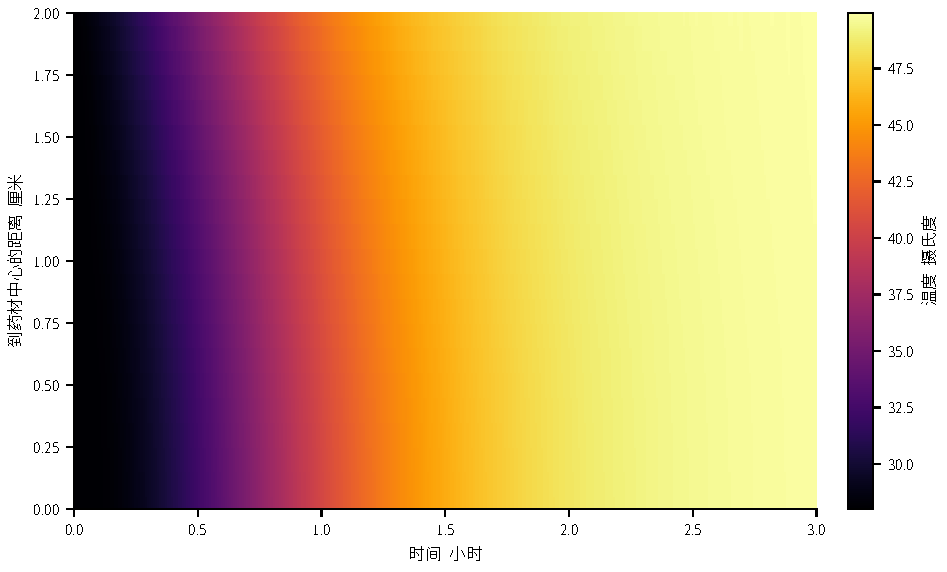
\includegraphics[width=0.92\textwidth]{figures/result_q2_temperature_field.pdf}
\caption{问题二前三小时的径向温度场}
\label{fig:q2-temperature}
\end{figure}

\begin{table}[htbp]
\centering
\caption{问题二指定时空点的干基含水率}
\label{tab:q2-moisture}
\begin{tabular}{cccccc}
\toprule
时间 & \multicolumn{5}{c}{不同半径处干基含水率 \si{kg/kg}}\\
\cmidrule(lr){2-6}
\si{h} & \SI{0}{cm} & \SI{0.5}{cm} & \SI{1.0}{cm} & \SI{1.5}{cm} & \SI{2.0}{cm}\\
\midrule
0.5 & 2.5499 & 2.5489 & 2.5255 & 2.3257 & 1.6486\\
1.0 & 2.5257 & 2.4948 & 2.3578 & 2.0230 & 1.4711\\
1.5 & 2.3861 & 2.3256 & 2.1344 & 1.8020 & 1.3476\\
2.0 & 2.1708 & 2.1084 & 1.9236 & 1.6259 & 1.2311\\
2.5 & 1.9566 & 1.9006 & 1.7360 & 1.4720 & 1.1166\\
3.0 & 1.7662 & 1.7165 & 1.5702 & 1.3333 & 1.0081\\
\bottomrule
\end{tabular}
\end{table}

\SI{0.5}{h} 时中心含水率为 \SI{2.5499}{kg/kg}，表面含水率已降至 \SI{1.6486}{kg/kg}。到 \SI{3}{h}，两处数值分别为 \SI{1.7662}{kg/kg} 和 \SI{1.0081}{kg/kg}，中心比表面高 \SI{0.7581}{kg/kg}。图 \ref{fig:q2-moisture} 显示低含水率区持续向内部扩展，轴线附近的扩散滞后仍未消失。

\begin{figure}[htbp]
\centering
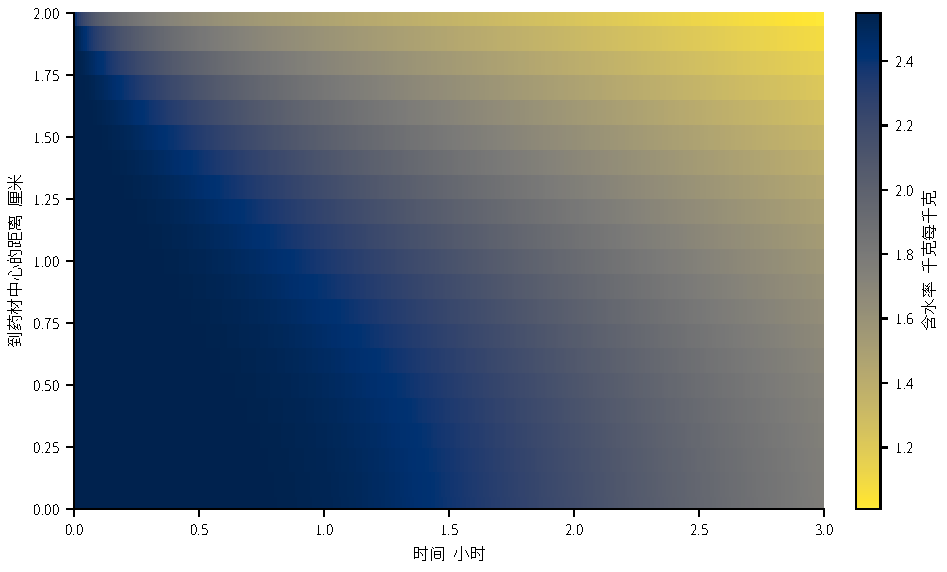
\includegraphics[width=0.92\textwidth]{figures/result_q2_moisture_field.pdf}
\caption{问题二前三小时的径向干基含水率场}
\label{fig:q2-moisture}
\end{figure}

\subsubsection{数值精度检验}

把时间步缩小至 \SI{0.5}{s} 后，指定时空点的温度和含水率最大绝对差分别为 \(1.9005\times10^{-6}\,\si{\degreeCelsius}\) 和 \(2.0140\times10^{-8}\,\si{kg/kg}\)，四位小数结果均未改变。把径向区间数增加至三百二十后，对应差值为 \(1.3031\times10^{-5}\,\si{\degreeCelsius}\) 和 \(1.1647\times10^{-5}\,\si{kg/kg}\)。温度表没有变化，含水率表仅有两个单元格的末位改变一个单位，全部差值低于四位小数舍入半单位 \(5\times10^{-5}\)。

水分离散平衡的最大相对残差为 \(1.6932\times10^{-11}\)。温度和含水率三对角系统的最大线性残差分别为 \(6.9221\times10^{-15}\) 和 \(7.5490\times10^{-16}\)，末时刻矩阵条件数分别为 \(2189.789\) 和 \(1243.281\)。这些结果说明局部守恒、线性求解和非线性迭代误差均小于结果表的输出精度。

换热系数取基准值的 \SI{80}{\percent} 和 \SI{120}{\percent} 时，温度最大变化分别为 \SI{1.0817}{\degreeCelsius} 和 \SI{0.7885}{\degreeCelsius}，含水率最大变化分别为 \SI{0.0154}{kg/kg} 和 \SI{0.0105}{kg/kg}。传质系数采用相同比例扰动时，温度最大变化为 \SI{0.0567}{\degreeCelsius} 和 \SI{0.0492}{\degreeCelsius}，含水率最大变化为 \SI{0.1694}{kg/kg} 和 \SI{0.1348}{kg/kg}。图 \ref{fig:q2-sensitivity} 显示温度主要受换热系数控制，含水率对传质系数更敏感。

\begin{figure}[htbp]
\centering
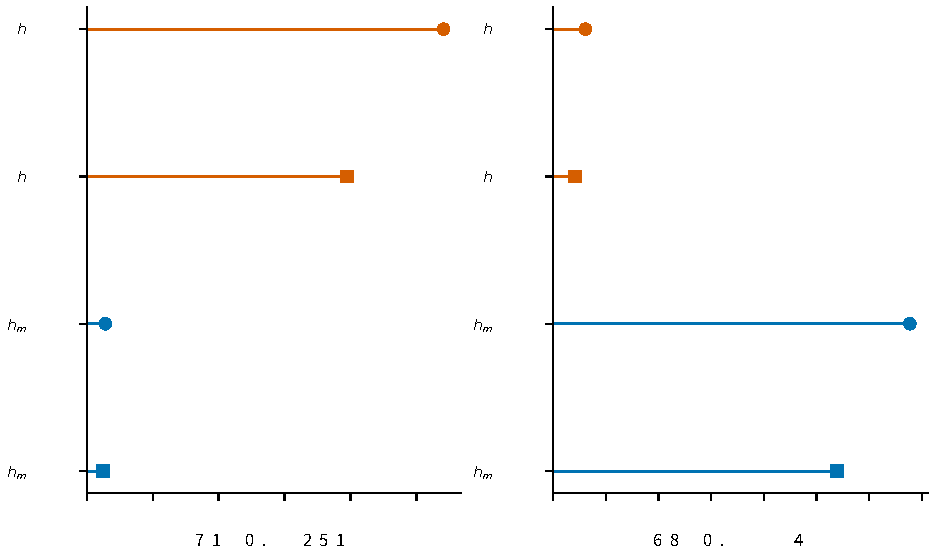
\includegraphics[width=0.92\textwidth]{figures/process_q2_sensitivity.pdf}
\caption{问题二边界参数的确定性灵敏度}
\label{fig:q2-sensitivity}
\end{figure}

\FloatBarrier

\subsection{问题三的固定域求解}

\subsubsection{稳定边界的取值}

附件一后段围绕平台水平波动。选取 \SI{9000}{s} 至 \SI{14400}{s} 的九十一个观测点，得到温度均值 \SI{50.004945}{\degreeCelsius}，总体标准差 \SI{0.154016}{\degreeCelsius}；空气水分浓度均值为 \SI{0.049993736}{kg/kg}，总体标准差为 \SI{0.000153463}{kg/kg}。

稳定段温度从 \SI{49.757}{\degreeCelsius} 变化至 \SI{50.246}{\degreeCelsius}，空气水分浓度从 \SI{0.04975}{kg/kg} 变化至 \SI{0.05025}{kg/kg}。这些观测量给出均值延拓的波动尺度，也为后续确定性敏感性检验提供扰动幅度。

已观测时段仍对附件数据作分段线性插值。后续边界取稳定段均值，写为
\begin{equation}
\left(T_a(t),C_a(t)\right)=
\begin{cases}
\left(T_{a,\mathrm{lin}}(t),C_{a,\mathrm{lin}}(t)\right), & 0\le t\le \SI{14400}{s},\\
\left(\SI{323.154945}{K},\SI{0.049993736}{kg/kg}\right), & t>\SI{14400}{s}.
\end{cases}
\label{eq:constant-air-boundary}
\end{equation}
式 \ref{eq:constant-air-boundary} 只固定烘房状态，药材内部场仍按非稳态方程推进。末条记录另作替代工况，用来量化边界取值对干燥时长的影响。

\subsubsection{全域阈值的事件判定}

问题三继承式 \ref{eq:q2-rho} 至式 \ref{eq:q2-properties} 的物性关系、式 \ref{eq:q2-fvm-unified} 的有限体积守恒式和式 \ref{eq:q2-surface-sources} 的表面通量。定义
\begin{equation}
C_{\max}(t)=\max_{0\le r\le R}C(r,t),\qquad
t_{\mathrm{dry}}^{\mathrm{fixed}}
=\inf\left\{t>0:C_{\max}(t)<0.15\right\}.
\label{eq:fixed-drying-end}
\end{equation}
式 \ref{eq:fixed-drying-end} 在全部径向节点上取最大值，不预设控制位置。早期近似均匀场存在数值并列，径向梯度形成后中心值等于全域最大值。

首个时间层用后向 Euler 格式，其余时间层采用式 \ref{eq:q2-bdf2} 的二阶向后差分。每层 Picard 迭代在温度最大变化不超过 \SI{1e-8}{\degreeCelsius} 且含水率最大变化不超过 \SI{1e-10}{kg/kg} 时停止，迭代上限为四十次。程序以 \SI{1}{s} 时间步检查式 \ref{eq:fixed-drying-end}，以 \SI{60}{s} 间隔写入结果，终点不落在常规记录时刻时单独追加。

空间网格采用三百二十个径向区间。输出表从 \SI{0}{cm} 到 \SI{2}{cm} 每隔 \SI{0.1}{cm} 给出含水率，加上时间列共二十二列。表内数值统一保留四位小数，完整文件含三千四百四十六条时间记录。

\subsubsection{固定尺寸下的干燥历程}

全域最大含水率在 \SI{206756}{s} 首次低于阈值，对应固定半径烘干时长 \SI{57.4322}{h}。前一常规记录 \SI{206700}{s} 的最大含水率为 \SI{0.15001607}{kg/kg}，终点值为 \SI{0.14999973}{kg/kg}。图 \ref{fig:q3-threshold} 给出全程轨迹和终点附近的局部变化，阈值跨越由中心含水率控制。

\begin{figure}[htbp]
\centering
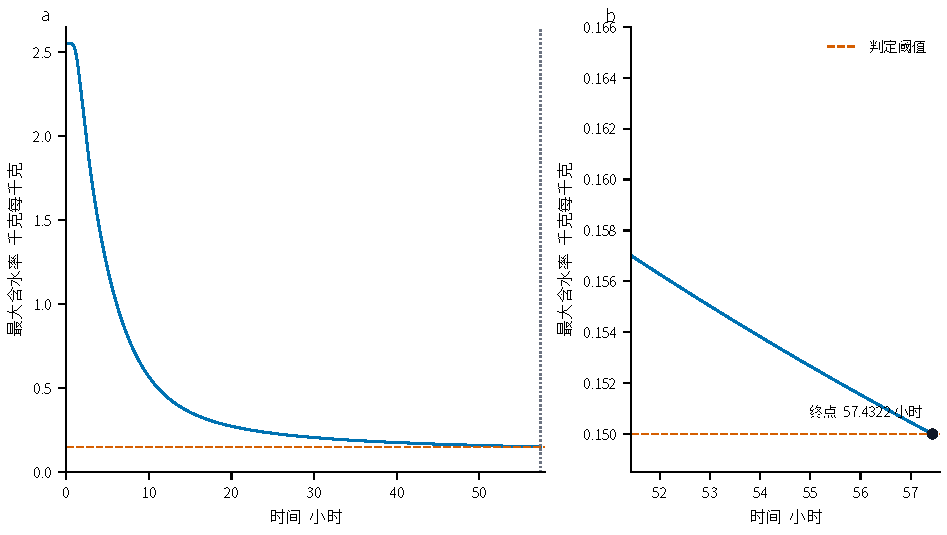
\includegraphics[width=0.94\textwidth]{figures/result_q3_threshold.pdf}
\caption{问题三全域最大含水率的首次阈值跨越}
\label{fig:q3-threshold}
\end{figure}

表 \ref{tab:q3-moisture} 列出每隔六小时及烘干结束时的五个指定位置结果。表面含水率在 \SI{18}{h} 已降至 \SI{0.0845}{kg/kg}，中心仍为 \SI{0.2988}{kg/kg}。到 \SI{54}{h}，中心含水率为 \SI{0.1538}{kg/kg}，离结束条件只差 \SI{0.0038}{kg/kg}。

\begin{table}[htbp]
\centering
\caption{问题三指定位置的干基含水率}
\label{tab:q3-moisture}
\begin{tabular}{cccccc}
\toprule
时间 & \multicolumn{5}{c}{不同半径处干基含水率 \si{kg/kg}}\\
\cmidrule(lr){2-6}
\si{h} & \SI{0}{cm} & \SI{0.5}{cm} & \SI{1.0}{cm} & \SI{1.5}{cm} & \SI{2.0}{cm}\\
\midrule
6.0000  & 1.0169 & 0.9881 & 0.9015 & 0.7550 & 0.5328\\
12.0000 & 0.4561 & 0.4431 & 0.4030 & 0.3297 & 0.1642\\
18.0000 & 0.2988 & 0.2915 & 0.2687 & 0.2253 & 0.0845\\
24.0000 & 0.2378 & 0.2327 & 0.2167 & 0.1855 & 0.0665\\
30.0000 & 0.2058 & 0.2018 & 0.1891 & 0.1640 & 0.0598\\
36.0000 & 0.1858 & 0.1825 & 0.1718 & 0.1503 & 0.0566\\
42.0000 & 0.1720 & 0.1691 & 0.1597 & 0.1406 & 0.0548\\
48.0000 & 0.1618 & 0.1591 & 0.1506 & 0.1334 & 0.0537\\
54.0000 & 0.1538 & 0.1514 & 0.1436 & 0.1276 & 0.0530\\
57.4322 & 0.1500 & 0.1477 & 0.1402 & 0.1249 & 0.0527\\
\bottomrule
\end{tabular}
\end{table}

终点行的中心值按题目要求显示为四位小数，未舍入值为 \SI{0.14999973}{kg/kg}，因此满足严格小于阈值的条件。图 \ref{fig:q3-profiles} 显示外层先进入低含水率区，中心曲线下降最慢。中心与表面的先后差异说明体积平均值不能替代全域判据。

\begin{figure}[htbp]
\centering
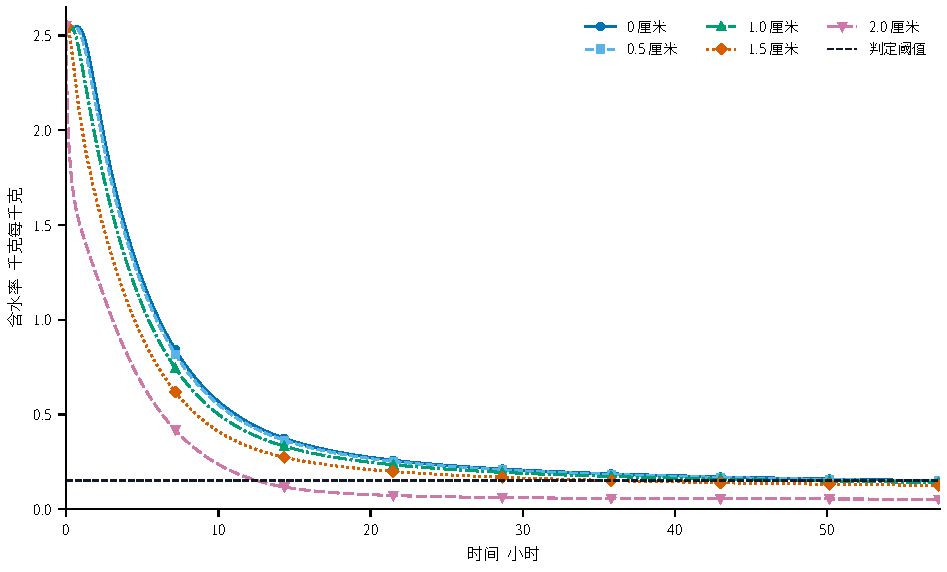
\includegraphics[width=0.90\textwidth]{figures/result_q3_profiles.pdf}
\caption{问题三五个指定径向位置的含水率历程}
\label{fig:q3-profiles}
\end{figure}

\subsubsection{数值可靠性检验}

时间步检验固定一百六十个径向区间。\SI{1}{s}、\SI{0.5}{s} 和 \SI{0.25}{s} 对应的烘干时长分别为 \SI{206569}{s}、\SI{206568.5}{s} 和 \SI{206568.5}{s}，前两者相对最细时间步的绝对差为 \SI{0.5}{s} 和零，分别满足 \SI{1}{s} 与 \SI{0.5}{s} 的预设门槛。空间检验固定 \SI{1}{s} 时间步，一百六十与三百二十区间的烘干时长相对差为 \SI{0.09044}{\percent}。指定表值的最大差为 \SI{1.0307e-4}{kg/kg}，超过四位小数舍入半单位，故最终取三百二十区间。

权威解的最大含水率反向增量为 \SI{3.9968e-15}{kg/kg}，水分平衡最大相对残差为 \(6.8716\times10^{-10}\)。温度与含水率线性系统的最大相对残差分别为 \(3.0249\times10^{-14}\) 和 \(2.4208\times10^{-15}\)，末时刻条件数分别为 \(8386.07\) 和 \(1771.93\)。全部时间层最多用四次 Picard 迭代，代数残差、守恒残差及层内迭代误差没有影响最终输出精度或终点判断。

稳定温度减少和增加一个总体标准差时，烘干时长分别变化 \SI{0.4904}{\percent} 和 \SI{-0.4875}{\percent}；空气水分浓度作相同方式扰动时，变化幅度不超过 \SI{0.0063}{\percent}。采用附件末条记录会使时长缩短 \SI{0.5117}{\percent}。按端面与侧面面积比把换热及传质系数同时放大 \SI{8}{\percent} 后，时长缩短 \SI{0.8372}{\percent}，低于预设的 \SI{8}{\percent} 回退门槛。图 \ref{fig:q3-sensitivity} 表明长期边界选择和端面简化对本问结论的影响均在百分之一以内。

\begin{figure}[htbp]
\centering
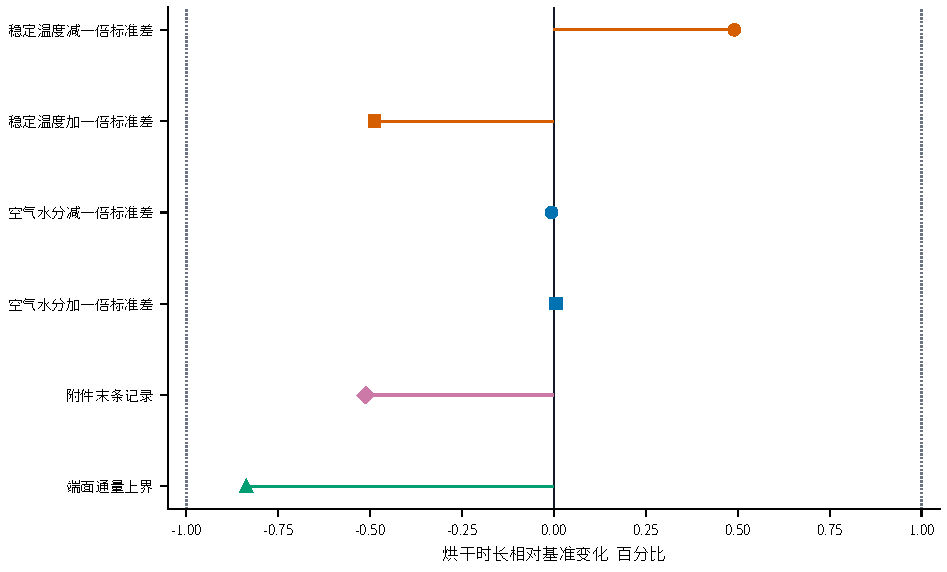
\includegraphics[width=0.92\textwidth]{figures/process_q3_boundary_sensitivity.pdf}
\caption{问题三长期边界及端面通量上界的确定性敏感性}
\label{fig:q3-sensitivity}
\end{figure}

\FloatBarrier

\subsection{问题四的收缩域求解}

\subsubsection{移动域控制方程}

附件二的半径记录覆盖零至七十二小时。全部一百四十五个观测点按时间顺序连接，半径由 \SI{2}{cm} 减小至 \SI{1.198}{cm}，收缩速度在后段趋近于零。计算在相邻记录间作分段线性插值，既保留观测值，又避免额外拟合参数。图 \ref{fig:q4-radius} 给出模型实际调用的半径边界。

设相邻观测点为 \((t_j,R_j)\) 和 \((t_{j+1},R_{j+1})\)，计算中的半径边界取
\begin{equation}
R(t)=R_j+\frac{R_{j+1}-R_j}{t_{j+1}-t_j}(t-t_j),
\qquad t_j\leq t\leq t_{j+1}.
\label{eq:q4-radius-interpolation}
\end{equation}
该式在每个观测时刻严格返回附件记录值，主模型终点位于观测区间内，不需要对半径作区间外延拓。

\begin{figure}[htbp]
\centering
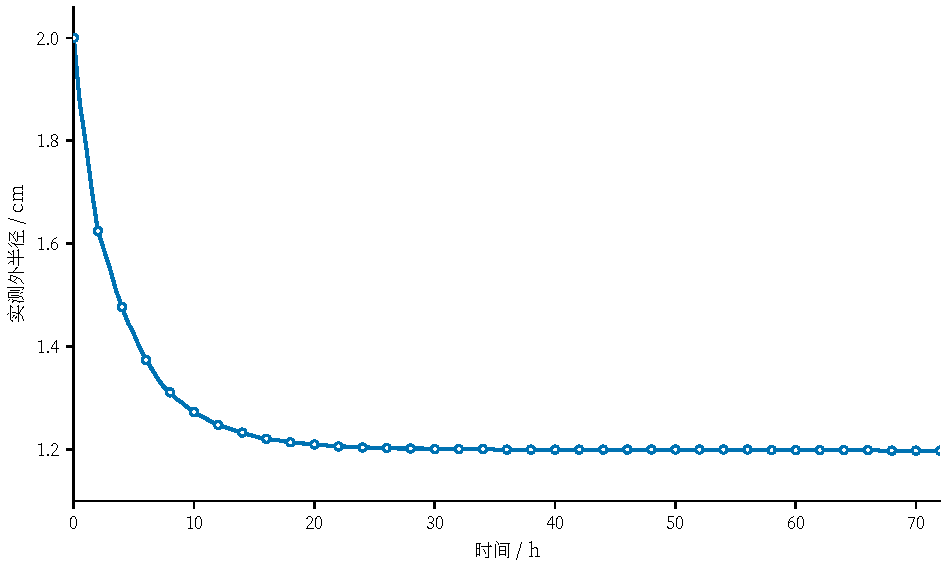
\includegraphics[width=0.90\textwidth]{figures/raw_q4_radius.pdf}
\caption{附件二半径记录构成的移动边界}
\label{fig:q4-radius}
\end{figure}
\FloatBarrier

固定物理坐标会随外表面内移而退出药材区域。食品干燥研究可在移动坐标中统一描述内部传递和几何变化\cite{adrover2019general}。为保持网格拓扑不变，令
\begin{equation}
x=\frac{r}{R(t)},\qquad 0\leq x\leq 1,
\label{eq:normalized-radius}
\end{equation}
材料坐标中的温度及干基含水率分别记为 \(\widetilde{T}(x,t)\) 和 \(\widetilde{C}(x,t)\)。相似收缩下的\mbox{径向速度}为
\begin{equation}
v_r(r,t)=\frac{rR'(t)}{R(t)}.
\label{eq:material-velocity}
\end{equation}
固定 \(x\) 的时间导数就是物理场的材料导数
\begin{equation}
\left.\frac{\partial \widetilde{u}}{\partial t}\right|_{x}
=
\left.\frac{\partial u}{\partial t}\right|_{r}
+v_r\frac{\partial u}{\partial r}.
\label{eq:material-derivative}
\end{equation}
式中 \(u\) 表示温度或含水率。该坐标变换把随时间变化的物理域转化为固定单位区间，移动项在材料导数中得到处理。

温度和水分仍服从前文采用的有效扩散机制。坐标变换后的方程为
\begin{align}
\rho c_p\frac{\partial \widetilde{T}}{\partial t}
&=
\frac{1}{xR^2(t)}
\frac{\partial}{\partial x}
\left(
xk\frac{\partial \widetilde{T}}{\partial x}
\right),
\label{eq:moving-heat}\\
\frac{\partial \widetilde{C}}{\partial t}
&=
\frac{1}{xR^2(t)}
\frac{\partial}{\partial x}
\left(
xD\frac{\partial \widetilde{C}}{\partial x}
\right).
\label{eq:moving-moisture}
\end{align}
其中 \(R^{-2}(t)\) 表示扩散距离缩短产生的几何作用。中心保持零通量，表面边界为
\begin{align}
-\frac{k}{R(t)}\left.\frac{\partial\widetilde{T}}{\partial x}\right|_{x=1}
&=h\left[\widetilde{T}(1,t)-T_a(t)\right],\\
-\frac{D}{R(t)}\left.\frac{\partial\widetilde{C}}{\partial x}\right|_{x=1}
&=h_m\left[\widetilde{C}(1,t)-C_a(t)\right].
\label{eq:moving-boundaries}
\end{align}

附录四给出的物性关系随局部状态更新
\begin{align}
\rho(C)&=760+90C,\\
c_p(C)&=1850+2150\frac{C}{C+1},\\
k(C)&=0.12+0.20\frac{C}{C+1},\\
D(C,T)&=4.2\times10^{-4}
\exp\left(-\frac{0.30}{C}\right)
\exp\left(-\frac{3850}{T}\right).
\label{eq:q4-properties}
\end{align}
扩散系数中的温度取 K。空气边界沿用问题三的实测插值和稳定段均值，换热系数与传质系数保持不变，使问题四只引入附录四物性和半径边界。

\subsubsection{内部映射检验}

附件二只记录外半径，无法由题面唯一确定内部材料点的位移。相似收缩作为主模型闭合，不把局部密度反演成真实干固体运动。为检验这一闭合对终点的影响，引入初始材料坐标 \(\xi\)，并构造保持同一外半径的映射族
\begin{align}
r(\xi,t)&=R(t)\left[\xi+a_*g(t)\xi(1-\xi)\right],
\label{eq:q4-nonuniform-map}\\
g(t)&=\frac{1-R(t)/R_0}{1-R_{\mathrm{end}}/R_0},\\
r_\xi&=R(t)\left[1+a_*g(t)(1-2\xi)\right].
\label{eq:q4-map-jacobian}
\end{align}
映射在中心取零，在表面取 \(R(t)\)。参数 \(a_*\) 取零、0.1 和 0.2，计算区间内均有 \(r_\xi>0\)，材料点的径向顺序保持不变。

一般映射下的热质方程可写为统一形式
\begin{equation}
b\frac{\partial u}{\partial t}
=
\frac{1}{r r_\xi}
\frac{\partial}{\partial\xi}
\left(
\frac{r\Gamma}{r_\xi}
\frac{\partial u}{\partial\xi}
\right),
\label{eq:q4-general-map}
\end{equation}
温度方程取 \(b=\rho c_p\)、\(u=T\) 和 \(\Gamma=k\)，水分方程取 \(b=1\)、\(u=C\) 和 \(\Gamma=D\)。当 \(a_*=0\) 时，式 \ref{eq:q4-general-map} 退化为式 \ref{eq:moving-heat} 及式 \ref{eq:moving-moisture}，三个情景属于同一模型族。

\clearpage

固定尺寸对照同样采用附录四物性、空气边界、初始条件和数值算法，仅将半径\mbox{恒定}为初始值 \(R_0\)。设相似收缩时长为 \(t_{\mathrm{dry}}^{(4)}\)，固定尺寸时长为 \(t_{\mathrm{dry}}^{(4,0)}\)，净几何效应定义为
\begin{equation}
\eta_R=
\frac{t_{\mathrm{dry}}^{(4)}-t_{\mathrm{dry}}^{(4,0)}}
{t_{\mathrm{dry}}^{(4,0)}}\times100\%.
\label{eq:q4-geometry-effect}
\end{equation}
该对照只关闭半径变化，不使用问题三的物性结果，因而能够分离附录四体系内的几何贡献。

\subsubsection{离散求解}

单位材料区间划分为三百二十个径向控制体。控制体体积和控制面面积在每个时间层按当前映射更新，内部通量在相邻控制体间取相反符号。首个时间层采用后向 Euler 格式，其余时间层采用式 \ref{eq:q2-bdf2} 的二阶向后差分，正式时间步为 \SI{1}{s}。

记第 \(i\) 个控制体的环形体积权重为 \(w_i^n\)，相邻节点间的扩散导通系数为 \(G_{i+1/2}^n\)。统一变量 \(u\) 的离散方程写为
\begin{align}
w_i^n&=\frac{\left(r_{i+1/2}^n\right)^2-\left(r_{i-1/2}^n\right)^2}{2},\\
G_{i+1/2}^n&=
\frac{r_{i+1/2}^n\Gamma_{i+1/2}^n}
{r_{i+1}^n-r_i^n},\\
\frac{b_i^n w_i^n}{\Delta t_{\mathrm{eff}}}
\left(u_i^n-H_{u,i}^n\right)
&=G_{i-1/2}^n\left(u_{i-1}^n-u_i^n\right)
+G_{i+1/2}^n\left(u_{i+1}^n-u_i^n\right).
\label{eq:q4-fvm}
\end{align}
首层取 \(H_{u,i}^n=u_i^{n-1}\) 和 \(\Delta t_{\mathrm{eff}}=\Delta t\)，后续时间层取 \(H_{u,i}^n=(4u_i^{n-1}-u_i^{n-2})/3\) 和 \(\Delta t_{\mathrm{eff}}=2\Delta t/3\)。表面控制体再加入 \(R^n\beta(u_N^n-u_a^n)\)，温度和水分方程中的 \(\beta\) 分别取 \(h\) 和 \(h_m\)。

每个时间层先依据当前含水率更新 \(\rho\)、\(c_p\) 和 \(k\)，求得温度后再更新 \(D\) 并求解含水率。温度及含水率相邻两轮的最大绝对差分别低于 \(10^{-8}\,\si{\degreeCelsius}\) 和 \(10^{-10}\,\si{kg/kg}\) 时停止 Picard 迭代，迭代上限为四十次。主模型全部时间层最多迭代四次，其中九万三千四百四十九层用三次，九万零四百三十层用四次。

干燥终点在每个内部时间步检查，定义为
\begin{equation}
t_{\mathrm{dry}}^{(4)}
=
\inf\left\{
t>0:
\max_{0\leq x\leq 1}\widetilde{C}(x,t)<0.15
\right\}.
\label{eq:shrink-drying-end}
\end{equation}
结果文件每隔 \SI{60}{s} 保存一次，并额外保存终点。固定实际位置通过 \(x=r/R(t)\) 映射到当前网格，超出当前半径的位置记为域外，独立末列始终记录药材表面。

\subsubsection{干燥终点结果}

主模型在 \SI{183879}{s} 首次满足全域严格阈值，对应 \SI{51.0775}{h}。前一秒的最大含水率为 \SI{0.150000202481}{kg/kg}，终点值为 \SI{0.149999688772}{kg/kg}，控制位置位于轴线。

计算终点的半径为 \SI{1.2000}{cm}，早于附件二七十二小时观测结束时刻，计算没有使用半径末值延拓。

把两次判定值减去阈值可得
\begin{equation}
\Delta C_{\mathrm{pre}}=2.02481\times10^{-7}>0,
\qquad
\Delta C_{\mathrm{end}}=-3.11228\times10^{-7}<0.
\label{eq:q4-threshold-crossing}
\end{equation}
符号变化表明终点由未舍入结果确定，表 \ref{tab:q4-moisture} 中显示的四位小数不参与阈值判定。

图 \ref{fig:q4-moisture} 显示低含水率区域由表面向轴线推进，药材区域随外表面内移而缩小。白色部分表示固定物理位置已经位于药材域外，不属于数据缺失。径向梯度在后段减弱，中心始终是最晚越过阈值的位置。

\begin{figure}[htbp]
\centering
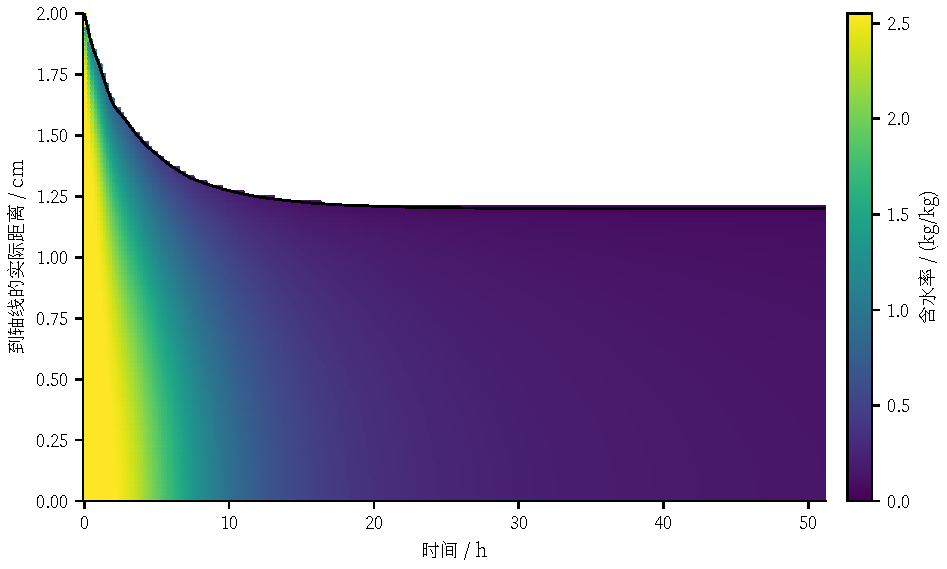
\includegraphics[width=0.92\textwidth]{figures/result_q4_moving_field.pdf}
\caption{收缩域内干基含水率的时空演化}
\label{fig:q4-moisture}
\end{figure}

表 \ref{tab:q4-moisture} 给出六小时间隔及终点处的代表性结果。六小时至终点期间，半径由 \SI{1.3740}{cm} 减小至 \SI{1.2000}{cm}，中心含水率由 \SI{1.7195}{kg/kg} 降至阈值以下。固定位置 \SI{1.5}{cm} 在这些时刻均位于药材域外，表面值另列，避免把被收缩移出的空间点误写成表面值。

\begin{table}[htbp]
\centering
\caption{考虑尺寸收缩的药材干基含水率}
\label{tab:q4-moisture}
\small
\begin{tabular}{ccccccc}
\toprule
时间 \si{h} & 半径 \si{cm} & \SI{0}{cm} & \SI{0.5}{cm} & \SI{1.0}{cm} & \SI{1.5}{cm} & 药材表面\\
\midrule
6.0000  & 1.3740 & 1.7195 & 1.5377 & 1.0226 & 域外 & 0.4207\\
12.0000 & 1.2480 & 0.7376 & 0.6545 & 0.4083 & 域外 & 0.1669\\
18.0000 & 1.2140 & 0.4087 & 0.3686 & 0.2397 & 域外 & 0.0892\\
24.0000 & 1.2040 & 0.2851 & 0.2610 & 0.1790 & 域外 & 0.0673\\
30.0000 & 1.2010 & 0.2263 & 0.2093 & 0.1492 & 域外 & 0.0595\\
36.0000 & 1.2000 & 0.1928 & 0.1796 & 0.1316 & 域外 & 0.0560\\
42.0000 & 1.2000 & 0.1712 & 0.1603 & 0.1199 & 域外 & 0.0541\\
48.0000 & 1.2000 & 0.1561 & 0.1468 & 0.1115 & 域外 & 0.0530\\
51.0775 & 1.2000 & 0.1500 & 0.1413 & 0.1081 & 域外 & 0.0526\\
\bottomrule
\end{tabular}
\par\smallskip{\footnotesize 终点中心值按四位小数显示为 0.1500，判定使用的未舍入值严格小于 0.15。}
\end{table}

同附录四物性的固定半径对照在 \SI{467267}{s} 达到阈值，对应 \SI{129.7964}{h}。式 \ref{eq:q4-geometry-effect} 给出 \(\eta_R=-60.6480\%\)，即观测半径收缩使模型终点缩短 \SI{78.7189}{h}。图 \ref{fig:q4-comparison} 显示两个情景使用同一阈值，却因扩散距离不同而在相隔 \SI{283388}{s} 的时刻结束。

计算结果代入几何效应指标后得到
\begin{equation}
\Delta t_R=t_{\mathrm{dry}}^{(4)}-t_{\mathrm{dry}}^{(4,0)}
=-\SI{78.7189}{h},
\qquad
\eta_R=-60.6480\%.
\label{eq:q4-geometry-result}
\end{equation}
该式中的时间差只反映半径边界变化，物性、空气边界和离散参数均保持相同。

\begin{figure}[htbp]
\centering
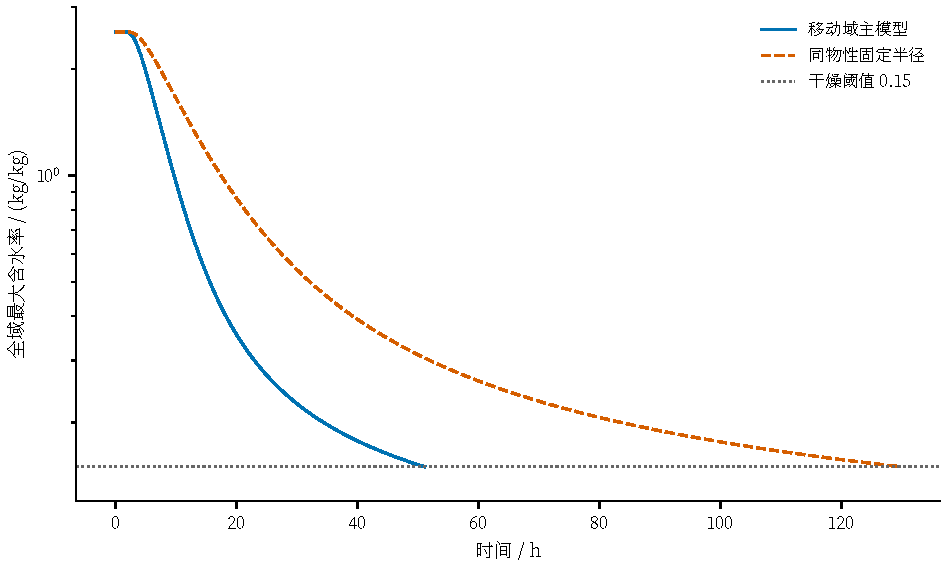
\includegraphics[width=0.92\textwidth]{figures/result_q4_threshold.pdf}
\caption{收缩域主模型和固定半径对照的阈值跨越}
\label{fig:q4-comparison}
\end{figure}

\subsubsection{数值精度检验}

内部映射参数取 0.1 和 0.2 时，干燥时长分别为 \SI{51.1572}{h} 和 \SI{51.2381}{h}。相对主模型的变化为 \SI{0.1561}{\percent} 和 \SI{0.3143}{\percent}，最大结构偏差为 \SI{0.3143}{\percent}。图 \ref{fig:q4-shape} 表明两组未校准的确定性情景均保持同一实测外半径，所得时长变化不超过十分钟。

记参数为 \(a_*\) 时的干燥时长为 \(t_{\mathrm{dry}}(a_*)\)。内部映射的相对时长变化和最大结构偏差定义为
\begin{equation}
\eta_a(a_*)=
\frac{t_{\mathrm{dry}}(a_*)-t_{\mathrm{dry}}(0)}
{t_{\mathrm{dry}}(0)}\times100\%,
\qquad
E_{\mathrm{shape}}=\max_{a_*\in\{0.1,0.2\}}|\eta_a(a_*)|.
\label{eq:q4-shape-error}
\end{equation}
其中 \(a_*=0\) 对应相似收缩主映射。两组计算给出 \(E_{\mathrm{shape}}=0.3143\%\)。

\begin{figure}[htbp]
\centering
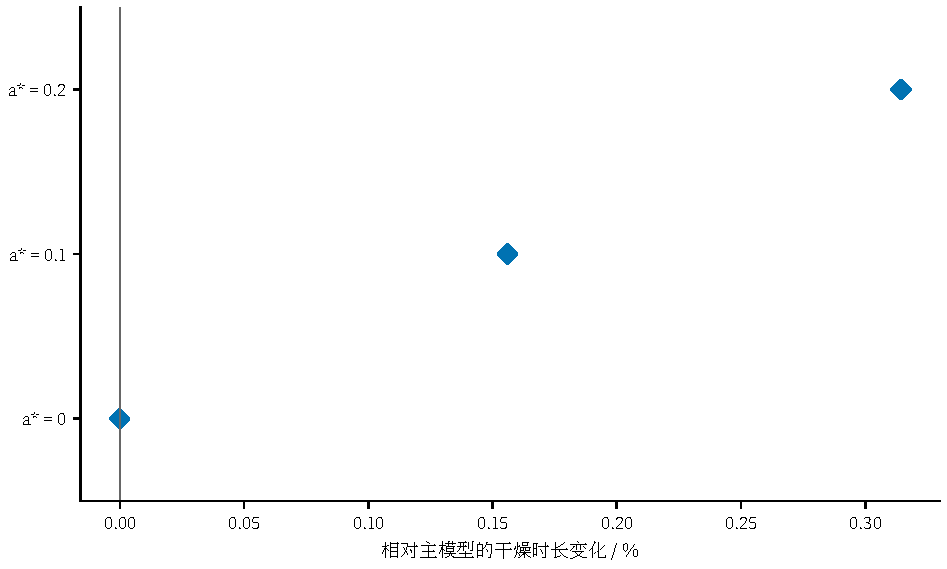
\includegraphics[width=0.88\textwidth]{figures/result_q4_shape_sensitivity.pdf}
\caption{内部收缩映射对干燥时长的确定性影响}
\label{fig:q4-shape}
\end{figure}
\FloatBarrier

空间网格增至六百四十个区间后，终点相差 \SI{13}{s}，相对差为 \SI{0.007069}{\percent}，共同表值最大差为 \(1.715844\times10^{-5}\,\si{kg/kg}\)。时间步减至 \SI{0.5}{s} 后，终点相差 \SI{0.5}{s}，共同表值最大差为 \(8.575106\times10^{-8}\,\si{kg/kg}\)。图 \ref{fig:q4-refinement} 将两类加密误差与四位小数的预定表值门槛比较，全部误差均低于 \(5\times10^{-5}\,\si{kg/kg}\)。

令 \(\mathcal S\) 表示两组结果共有的表格时刻和有效物理位置，网格误差与时间步误差取
\begin{align}
E_C^{N}&=\max_{(r,t)\in\mathcal S}
\left|C_{320}(r,t)-C_{640}(r,t)\right|,\\
E_C^{\Delta t}&=\max_{(r,t)\in\mathcal S}
\left|C_{1\,\mathrm{s}}(r,t)-C_{0.5\,\mathrm{s}}(r,t)\right|,\\
E_t&=\frac{|t_{\mathrm{dry}}^{\mathrm{coarse}}-t_{\mathrm{dry}}^{\mathrm{fine}}|}
{t_{\mathrm{dry}}^{\mathrm{fine}}}\times100\%.
\label{eq:q4-refinement-error}
\end{align}
该定义排除已经离开收缩域的固定位置，不把结构空值计作数值误差。

\begin{figure}[htbp]
\centering

\includegraphics[width=0.88\textwidth]{figures/process_q4_refinement.pdf}
\caption{问题四时间步和空间网格加密误差}
\label{fig:q4-refinement}
\end{figure}
\FloatBarrier

两类加密试验的统一判定量为
\begin{equation}
E_C^{\max}=\max\left\{E_C^N,E_C^{\Delta t}\right\}
=1.715844\times10^{-5}<5\times10^{-5}\,\si{kg/kg}.
\label{eq:q4-refinement-pass}
\end{equation}
该不等式说明表 \ref{tab:q4-moisture} 保留四位小数时，网格和时间步误差均未越过预定门槛。
\clearpage

水分和热量的离散平衡残差分别写为
\begin{align}
\mathcal B_C^n&=\sum_i w_i^n\delta_t C_i^n
+R^n h_m\left(C_N^n-C_a^n\right),\\
\mathcal B_T^n&=\sum_i \rho_i^n c_{p,i}^n w_i^n\delta_t T_i^n
+R^n h\left(T_N^n-T_a^n\right).
\label{eq:q4-balance-residual}
\end{align}
程序按储存项和边界项的量级归一化 \(\mathcal B_C^n\)，并用各热量项绝对量之和归一化 \(\mathcal B_T^n\)。线性方程组的相对残差采用
\begin{equation}
\varepsilon_{\mathrm{lin},u}=
\max_n\frac{\|A_u^n u^n-b_u^n\|_\infty}{\|b_u^n\|_\infty}.
\label{eq:q4-linear-residual}
\end{equation}
水分方程的离散平衡相对残差为 \(1.7883\times10^{-11}\)，热方程归一残差为 \(9.7424\times10^{-16}\)。热量和水分线性系统的最大相对残差分别为 \(3.5831\times10^{-14}\) 和 \(1.2016\times10^{-15}\)。该组残差检验有效扩散方程的离散一致性，不表示真实干固体和水分总质量守恒。

\section{模型评价}

\subsection{结构特点}

一维径向控制体直接对应题目要求的空间坐标，环形体积和控制面面积保留了圆柱几何特征。中心控制体的内表面积为零，无需在 \(r=0\) 处直接计算 \(1/r\)，离散后的每个方程仍保持局部守恒。

变物性模型把温度和含水率通过扩散系数及热物性联系起来，能够从预热阶段连续推进到恒温阶段。移动坐标把收缩域转化为固定单位区间，避免反复增删网格，并使问题三和问题四采用同一终点判据。

题面数据直接构成时间边界和半径边界，模型没有为缺失的实验量拟合额外参数。分段线性插值保持原始记录值，结果文件所需的时间和空间分辨率可以由数值网格直接输出。

\subsection{适用边界}

径向模型忽略端面传递，面积比只能说明端部贡献受限，不能证明所有轴向位置都满足相同场分布。一维模型和二维模型可能给出不同的局部场分布\cite{adrover2019dimensional}。靠近端面的温度和含水率需用二维模型抽样或端部测温数据评估偏差。

问题一把潜热和材料收缩排除在温度方程外，问题二至问题四也用等效扩散系数概括复杂的相变及孔隙输运。若蒸发潜热占热量收支的比例较高，当前温度预测会偏快。药材干基含水率与空气含湿量的基准物质可能不同，直接作差的传质边界需要结合题意和结果范围复核。

问题三的长时空气边界采用稳定段均值。总体标准差扰动和末条记录替代使终点时长变化不超过 \SI{0.5117}{\percent}。问题四五个情景的最大时长偏差为 \SI{0.5058}{\percent}。

主模型在 \SI{51.0775}{h} 结束，早于半径观测终点，因而没有调用末值保持规则。

问题四只观测外表面半径，内部映射参数没有实验标定。两组结构扰动把时长最多改变 \SI{0.3143}{\percent}，该数值只适用于式 \ref{eq:q4-nonuniform-map} 给出的映射族。模型若需描述局部孔隙演化和相变潜热，应增加内部位移及热质通量观测，再建立多相传递方程。

\CumcmAIUsed{模型一致性核查、程序调试、图表制作、论文结构起草、语言校核及 \LaTeX{} 排版}

\begingroup
\raggedright
\begin{thebibliography}{99}

\bibitem{tzempelikos2015}
TZEMPELIKOS D A, MITRAKOS D, VOUROS A P, et al.
Numerical modeling of heat and mass transfer during convective drying of cylindrical quince slices[J].
Journal of Food Engineering, 2015, 156: 10--21.
DOI: 10.1016/j.jfoodeng.2015.01.017.

\bibitem{silva2014}
DA SILVA W P, E SILVA C M D P S, GAMA F J A.
Estimation of thermo-physical properties of products with cylindrical shape during drying: The coupling between mass and heat[J].
Journal of Food Engineering, 2014, 141: 65--73.
DOI: 10.1016/j.jfoodeng.2014.05.010.

\bibitem{hussain2003}
HUSSAIN M M, DINCER I.
Two-dimensional heat and moisture transfer analysis of a cylindrical moist object subjected to drying: A finite-difference approach[J].
International Journal of Heat and Mass Transfer, 2003, 46(21): 4033--4039.
DOI: 10.1016/S0017-9310(03)00229-1.

\bibitem{liu2020}
刘格含, 王鹏, 吴小华, 等.
农产品热风干燥传热传质数值模拟研究进展[J].
食品工业科技, 2020, 41(22): 342--350, 357.
DOI: 10.13386/j.issn1002-0306.2020010245.

\bibitem{adrover2019general}
ADROVER A, BRASIELLO A, PONSO G.
A moving boundary model for food isothermal drying and shrinkage: General setting[J].
Journal of Food Engineering, 2019, 244: 178--191.
DOI: 10.1016/j.jfoodeng.2018.09.018.

\bibitem{adrover2019dimensional}
ADROVER A, BRASIELLO A.
A moving boundary model for food isothermal drying and shrinkage: One-dimensional versus two-dimensional approaches[J].
Journal of Food Process Engineering, 2019, 42(6): e13178.
DOI: 10.1111/jfpe.13178.

\end{thebibliography}
\endgroup

\clearpage
\begin{appendices}

\section{支撑材料清单}

% 待补：在程序、结果表、正式图和 AI 工具使用详情全部冻结后，
% 按最终提交包中的真实文件名填写支撑材料清单。

\section{计算程序}

% 待补：放入能够从题目附件复现 result1.xlsx 至 result4.xlsx 的完整源程序。
% 程序必须与论文公式、参数、时间步、空间步及最终结果保持一致。

\section{人工核验记录}

% 待补：AI 工具使用详情单独生成 AI工具使用详情.pdf 并放入支撑材料。
% 论文附录只保留组委会要求的文件清单和完整源程序，不写内部质检流程。

\end{appendices}

\end{document}
